\documentclass{article}
\usepackage{tikz}
\usetikzlibrary{angles, quotes}
\usepackage{amssymb}
\usepackage{pgfplots}
\pgfplotsset{width=10cm,compat=1.9}
\usepgfplotslibrary{statistics}
\usepackage[left=2.54cm,right=2.54cm,top=2.54cm,bottom=2.54cm]{geometry}
\usepackage{tasks} %Paquete necesario para la producción de items horizontales para algunos ejercicios de tarea empleando el comando /begin{multicols}}{#}.../end{multicols} para ayudarnos a reducir las páginas
\usepackage{pdflscape} %comando que permite cambiar a orientación horizontal las hojas%
\usepackage{soul} %Paquete para permitir la compilación de acentos usando el comando {\hl{}}}\\
\sethlcolor{yellow(munsell)} %comando para definir el color para el subrayado usando el comando \hl
\usepackage[utf8]{inputenc}
\usepackage[spanish]{babel}
\usepackage{icomma}
\usepackage{ragged2e}
\usepackage{siunitx}
\usepackage{url}
\usepackage[colorlinks=true, urlcolor=blue,  linkcolor=black, citecolor=green]{hyperref}
\usepackage{pdfpages}
\usepackage{blindtext} %Paquete que genera texto ficticio (dummy text) con el comando: \blindtext
\usepackage{cancel} %in the preamble gives you four different modes of striking through: \cancel{text to cancel} draws a diagonal line (slash) through its argument, \bcancel{text to cancel} uses the negative slope (a backslash), \xcancel{text to cancel} draws an X (actually \cancel plus \bcancel), \cancelto{〈value〉}{〈expression〉} draws a diagonal arrow through the 〈expression〉pointing to the 〈value〉 (math-mode only)
\usepackage{csquotes}
\usepackage{afterpage}
\usepackage{parskip} 
\usepackage{float}
\usepackage{enumitem}
\usepackage{multicol}%Paquete que permite la creación aislada de columnas de texto. De esta forma se reduce la cantidad de páginas en nuestro documento
\usepackage{lipsum} %Paquete que genera texto de relleno al igual que \usepackage{blindtext}, se usa con el comando \lipsum[#-#] los #(hashtags) delimitan el número de páginas que deseamos ocupar del paquete lipsum para usarlos como relleno. 

% Definir el comando personalizado para la nota
\newcommand{\mynote}[1]{%
\begin{tikzpicture}[baseline=-0.75ex]
\node[draw, circle, fill=Apple Green!60, inner sep=2pt] (note) {\textbf{Nota:}};
\end{tikzpicture}%
\ \textit{#1}%
}

\newenvironment{Figura}
{\par\medskip\noindent\minipage{\linewidth}}
{\endminipage\par\medskip}
\usepackage{caption}
\usepackage[
backend=biber,
sorting=none,
url=true
]{biblatex} %bibliografía
\addbibresource{biblio.bib}
% Establecer el espacio entre las entradas de la bibliografía
\setlength{\bibitemsep}{1\baselineskip} % Puedes ajustar el valor según tus preferencias
\usepackage{amsmath,amsthm,amssymb,amsfonts}
\usepackage{pifont} %Permite la compilación del comando \xmark: es el símbolo de la tachita
\usepackage{mathtools} %permite la compilación de símbolos para matrices
\usepackage{empheq} %Paquete que se relaciona con \usepackage[most]{tcolorbox} para la creación de cuadros/cajas de colores para delimitar los resultados matemáticos o líneas de texto usando la línea de comando: \begin{empheq}[box={\mymath[colback=orange(webcolor)!70,drop lifted shadow]}]{equation*} \end{empheq}
\usepackage[most]{tcolorbox} %Paquete que se relaciona con \usepackage{empheq} para la creación de cuadros/cajas de colores para delimitar los resultados matemáticos o líneas de texto
\renewcommand{\qedsymbol}{$\blacksquare$}
\usetikzlibrary{positioning,decorations.pathreplacing} %Paquete que permite la compilación de llaves para cuadros sinópticos (brace diagram) 
\usepackage{schemata} %The schemata package is designed just for these brace diagrams
\usepackage{booktabs}

\newcommand\AB[2]{\schema{\schemabox{#1}}{\schemabox{#2}}} %comando o paquete necesario para crear cuadros sinópticos

\newtcbox{\mymath}[1][]{%
nobeforeafter, math upper, tcbox raise base,
enhanced, colframe=blue!30!black,
colback=blue!30, boxrule=1pt,
#1} %Comando importante para encasillar los resultados matemáticos en cajas de diferentes colores, se relaciona con los paquetes \usepackage{empheq} y \usepackage[most]{tcolorbox} 

\newenvironment{sysmatrix}[1]
{\left(\begin{array}{@{}#1@{}}}
{\end{array}\right)}
\newcommand{\ro}[1]{%
\xrightarrow{\mathmakebox[\rowidth]{#1}}%
}
\newlength{\rowidth}% row operation width
\AtBeginDocument{\setlength{\rowidth}{3em}}  %Comando importante para laproducción de lineas de operaciones entre matrices, método de Gauss o Gauss Jordan se relaciona con \newenvironment{sysmatrix}

%formato para cambiar el horario a español
\usepackage[spanish]{datetime2}
\DTMsetdatestyle{spanish}

\renewcommand{\today}{\DTMdisplaydate{\the\year}{\the\month}{\the\day }{-1}}
%%%%%%%%%%%%%%%%%%%%%%%%%%%%%%%%%%%%%%%%%

\usepackage{datetime}
\newcommand{\mycurrenttime}{\xxivtime}

%%%%%%%%%%%%%%%%%%%%%%%%%%%%%%%%%%%%%%%%%%%%%%%%%%%%%%%%%%%%%%%%%%%%%%%%%%%%%%%%%%%%%%%%%%%%%%%%%%%%%%%%%%%%%%%%%%%%%%%%%%%%%%%%%%%%%%%%%%%%%%%%%


%%%%%%%%%%%%%Caja de color para el título%%%%%%%%%%%%%%%%%%%%%%%%%%%%%%%%%%%%%%%%%%%%%%%%%%%%%%

\definecolor{myframecolor}{RGB}{1, 45, 75} % Prussian Blue
\definecolor{myboxcolor}{RGB}{0, 107, 92} % Apple Green

\newtcolorbox{mybox}{
enhanced,
colback=myboxcolor!7, % Color de fondo del cuadro
colframe=myframecolor, % Color del marco del cuadro
arc=0pt,
boxrule=1pt,
borderline west={2mm}{-10mm}{myframecolor}, % Borde en el lado izquierdo
sharp corners=southwest,
width=\linewidth,
before=\par\vspace{\bigskipamount}, % Espacio antes del cuadro
after=\par\vspace{\bigskipamount} % Espacio después del cuadro
}


\newcommand{\euler}{e} %Comando para producir letra e de euler
\newenvironment{remark}{\par\vfill\footnotesize % Vertical white space above the remark and smaller font size
\begin{list}{}{
	\leftmargin=80pt % Indentation on the left
	\rightmargin=60pt}\item\ignorespaces % Indentation on the right
\makebox[-2.5pt]{\begin{tikzpicture}[overlay]
		\node[draw=Horizon!60,line width=2.5pt,circle,fill=Horizon!25,font=\sffamily\bfseries,inner sep=4pt,outer sep=0pt] at (-19pt,5pt){\textcolor{Horizon}{Nota}};\end{tikzpicture}} % Blue Nota in a circle
\advance\baselineskip -1pt}{\end{list}\vskip5pt} % Tighter line spacing and white space after remark
\usepackage{graphicx}

\usepackage{titling}

\input{colores.tex}

%%Producir signos de cita textual``Asignatura''

\newcommand{\xmark}{\ding{55}} %%%comando que genera la tachita

\newenvironment{MyColorPar}[1]{%
\leavevmode\color{#1}\ignorespaces%
}{%
}%

%%%%%%%%%%%%%%%%%%% Título de la tarea, Nombre de alumno

\title{Clase \# 29 - Estado Sólido}
\author{\emph{JA} $\boldsymbol{\mid}$}
\date{\today}

%%%%%%%%%%%%%%%%%%% Datos de la Materia

\usepackage{fancyhdr}
\fancypagestyle{plain}{%  the preset of fancyhdr 
\fancyhf{} % clear all header and footer fields
\fancyfoot[R]{
\includegraphics[width=2cm]{LogoFCFMBUAP (1).png}}
\fancyfoot[L]{{\bfseries{\thedate{}}} a las {\bfseries{\mycurrenttime{}}} horas{} (GMT-6, H. Puebla de Zaragoza, Pue)}
\fancyhead[L]{Estado sólido}
\fancyhead[R]{\theauthor}
}
\makeatletter
\def\@maketitle{%
\newpage
\null
\vskip 1em%
\begin{center}%
\let \footnote \thanks
{\LARGE \@title \par}%
\vskip 1em%
%{\large \@date}%
\end{center}%
\par
\vskip 1em}
\makeatother

\usepackage{lipsum}  
\usepackage{cmbright}


%%%%%%%%%%%%%%%%%%%%%%%%%%%%%%%%%%%%%%%%%%%%%%%%%%%%%%%%%%%%%%%%%%%%%%%%%%%%%%%%%%%%%%%%%%%%%%%%%%%%%%%%%%%%%%%%%%%%%%%%%%%%%%%%%%%%%%%%%%%%%%%%%%%%%%%%%%%%%%%%%%%%%%%%%%%%%%%%%%%%%%%%%%%%%%%%%%%%%%

\begin{document}



\maketitle


%%%%%%%%%%%%%%%%%%% Datos del profesor, campus y aula

\begin{mybox}
\noindent\begin{tabular}{@{}ll}
	{\bfseries{Profesor}} & Dra. Ana Lilia González Ronquillo\\
	\textcolor{prussianblue}{\bfseries{Campus}} / \textcolor{trueblue}{\bfseries{Facultad}}  & \textcolor{prussianblue}{\bfseries{C.U. BUAP}} /  \textcolor{trueblue}{\bfseries{FCFM}} \\
	\textcolor{prussianblue}{\bfseries{Edificio}} /  \textcolor{trueblue}{\bfseries{Salón}}    & 	\textcolor{prussianblue}{\bfseries{FM9}} /  \textcolor{trueblue}{\bfseries{301}}   
\end{tabular} 
\end{mybox} \vspace{1cm}

\tableofcontents

\vspace{2cm}

\section{Desplazamiento de átomos en la cadena diátomica}


Esto fue de la clase anterior (\textbf{quedó de tarea, subirá una asignasión a classroom}
 
 \begin{figure}[H]
    \centering
    
\includegraphics[width=0.7\textwidth]{1.png} % ajusta el ancho según convenga
    \caption{Descripción clara y concisa de la figura.}
    \label{fig:mi_figura} % opcional: para usar con \ref{fig:mi_figura}
\end{figure}



 \begin{figure}[H]
    \centering
    
\includegraphics[width=0.7\textwidth]{2.png} % ajusta el ancho según convenga
    \caption{Descripción clara y concisa de la figura.}
    \label{fig:mi_figura} % opcional: para usar con \ref{fig:mi_figura}
\end{figure}



En $\omega^{+}$ 

$\bullet$ Está graficada la primera zona de \textbf{Brillouin}. Para la cadena diátomica $\in [\pi/a, \pi/a]$


Desde el 0 hasta el valor máximo le toca un valor de $k$. Cada valor de $k$ corresponde un modo de oscilación con cierta frecuencia.

Si tenemos $n$ atómos tendremos $n$ modos de oscilación. Esos modos tiene una frecuencia entre $0$ y ese máximo. Pero también pueden tomar la otra posibilidad (excitar el modo) con una frecuencia u otra, si podemos controlar la frecuencia, podemos controlar $k$, si controlamos $k$, podemos controlar la frecuencia.

\textbf{¿Por qué le llamamos banda?}

Para el caso de las oscilaciones en una red la llamamos la \textit{banda prohibida fonónica} o de las oscilaciones de la red.


Resulta que tenemos todo un conjunto de valores que puede formar un conjunto continuo. Decimos que va desde el valor máximo de la banda acústica hsta ael valor mínimo de la banda acústica. 

A esto le llamos el anchi de banda de frecuencias prohibidas. 

Asociamos a números complejos a energía que se absorbe y la onda no se propaga, asociar valores de $k$ complejos.

 \begin{figure}[H]
    \centering
    
\includegraphics[width=0.7\textwidth]{4.png} % ajusta el ancho según convenga
    \caption{Descripción clara y concisa de la figura.}
    \label{fig:mi_figura} % opcional: para usar con \ref{fig:mi_figura}
\end{figure}


\subsection{Vibraciones de una red cúbica simple}

Estudiaremos las vibraciones de una red $CS$ monoatómica. 

Hasta ahora hemos visto el caso de una dimensión, Es decir:

\begin{itemize}
\item[$\bullet$] 1-D (monoatómica)
\item[$\bullet$] 1-D (diatómica)
\end{itemize}


 ¿Cómo sería el caso para más dimensiones, i.e. 2-D? 

 \begin{figure}[H]
    \centering
    
\includegraphics[width=0.7\textwidth]{3.png} % ajusta el ancho según convenga
    \caption{Descripción clara y concisa de la figura.}
    \label{fig:mi_figura} % opcional: para usar con \ref{fig:mi_figura}
\end{figure}

La complejidad que sucede de pasar de 1-D a 2-D las cosas se complican, pero en 3-D se complican aún más. :v

\textbf{Nueva Bibliografía a checar}: \textit{Sólyióm}. Posiblemente en biblioteca digital se puede descargar algunos caps.

Considerando interacción a 1os y 2os vecinos (las diagonales del cubo cercano al átomo en el plano) respecto de un Átomo en la posición ($\hat{i}$, $\hat{j}$, $\hat{k}$).

Posiciones de los 6 1os vecinos : 

\[  (i\pm 1,j,k),\, \quad (i,j\pm 1,k),\, \quad (i,j,k\pm 1)  \]


Es decir:


 \begin{figure}[H]
    \centering
    
\includegraphics[width=0.7\textwidth]{5.png} % ajusta el ancho según convenga
    \caption{Descripción clara y concisa de la figura.}
    \label{fig:mi_figura} % opcional: para usar con \ref{fig:mi_figura}
\end{figure}

Posiciones de los 12 2os vecinos:

\[  (i\pm 1, j\pm 1, k), \, \quad ( i\pm1, j,k\pm 1 ), \, \quad (i,j\pm1)  \]


Tenemos en la componente $x$:

 \begin{figure}[H]
    \centering
    
\includegraphics[width=0.7\textwidth]{6.png} % ajusta el ancho según convenga
    \caption{Descripción clara y concisa de la figura.}
    \label{fig:mi_figura} % opcional: para usar con \ref{fig:mi_figura}
\end{figure}

De la imagen anterior se tienen las siguiente variables $\ldots$ $K_{1}$ = constante de resorte de primeros vecinos $\neq$ vector $k$



  \begin{figure}[H]
    \centering
    
\includegraphics[width=0.7\textwidth]{8.png} % ajusta el ancho según convenga
    \caption{Descripción clara y concisa de la figura.}
    \label{fig:mi_figura} % opcional: para usar con \ref{fig:mi_figura}
\end{figure}


 \begin{figure}[H]
    \centering
    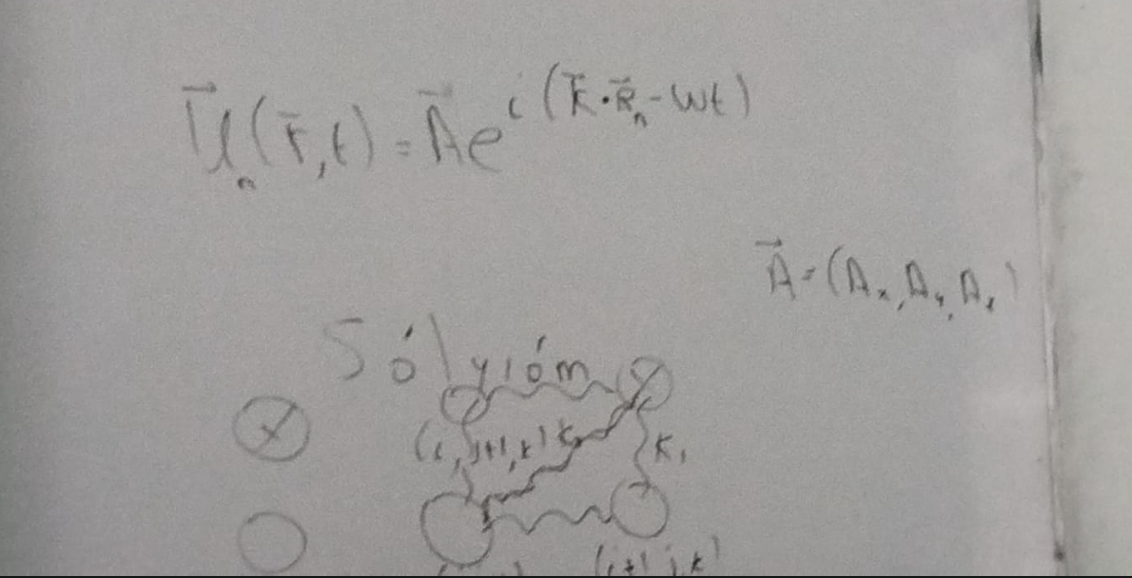
\includegraphics[width=0.7\textwidth]{9.png} % ajusta el ancho según convenga
    \caption{Descripción clara y concisa de la figura.}
    \label{fig:mi_figura} % opcional: para usar con \ref{fig:mi_figura}
\end{figure}

Extrapolado a 3-D:


 \begin{figure}[H]
    \centering
    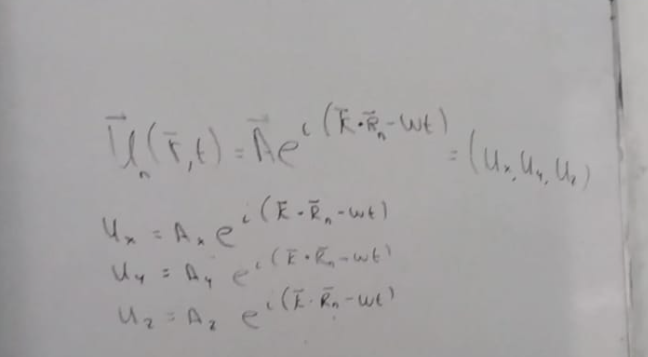
\includegraphics[width=0.7\textwidth]{10.png} % ajusta el ancho según convenga
    \caption{Descripción clara y concisa de la figura.}
    \label{fig:mi_figura} % opcional: para usar con \ref{fig:mi_figura}
\end{figure}

Podemos renombrar a $\alpha$ como:

\[  \alpha = 1,2,3 \quad \text{es decir} \quad \alpha = (x,y,z)\]

Se usa lo mismo que hicimos en la monoatomica, segunda ley de Newton. Juntamos todo y llegamos a esto:



 \begin{figure}[H]
    \centering
    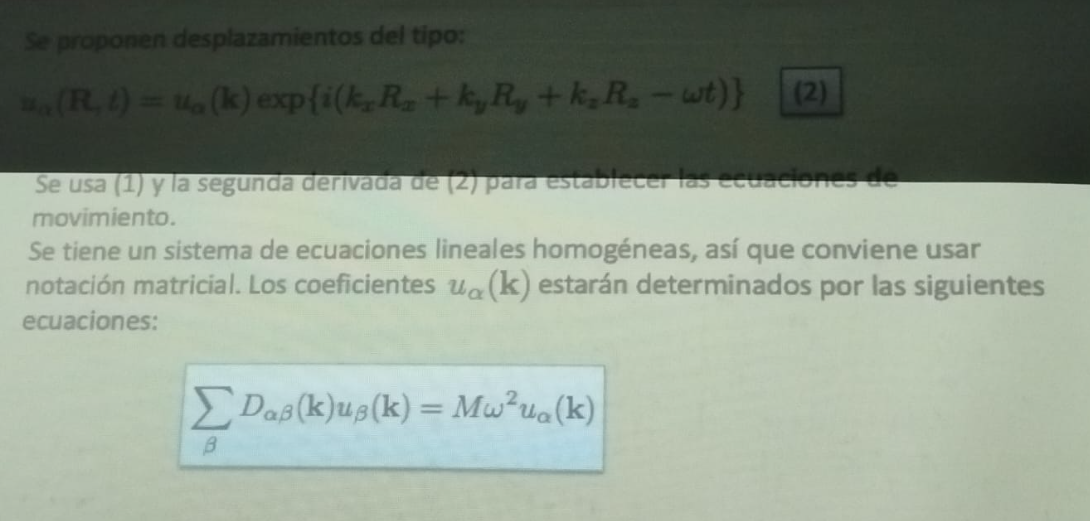
\includegraphics[width=0.7\textwidth]{11.png} % ajusta el ancho según convenga
    \caption{Descripción clara y concisa de la figura.}
    \label{fig:mi_figura} % opcional: para usar con \ref{fig:mi_figura}
\end{figure}


\textbf{Notación matricial anterior} (imagen anterior)


Tenemos a la segunda Ley de Newton:

\[ M\omega^{2}u_{\alpha}(\mathbf{k}) \quad \to \quad 2nd Newtons Law \]


Tenemos:

 \begin{figure}[H]
    \centering
    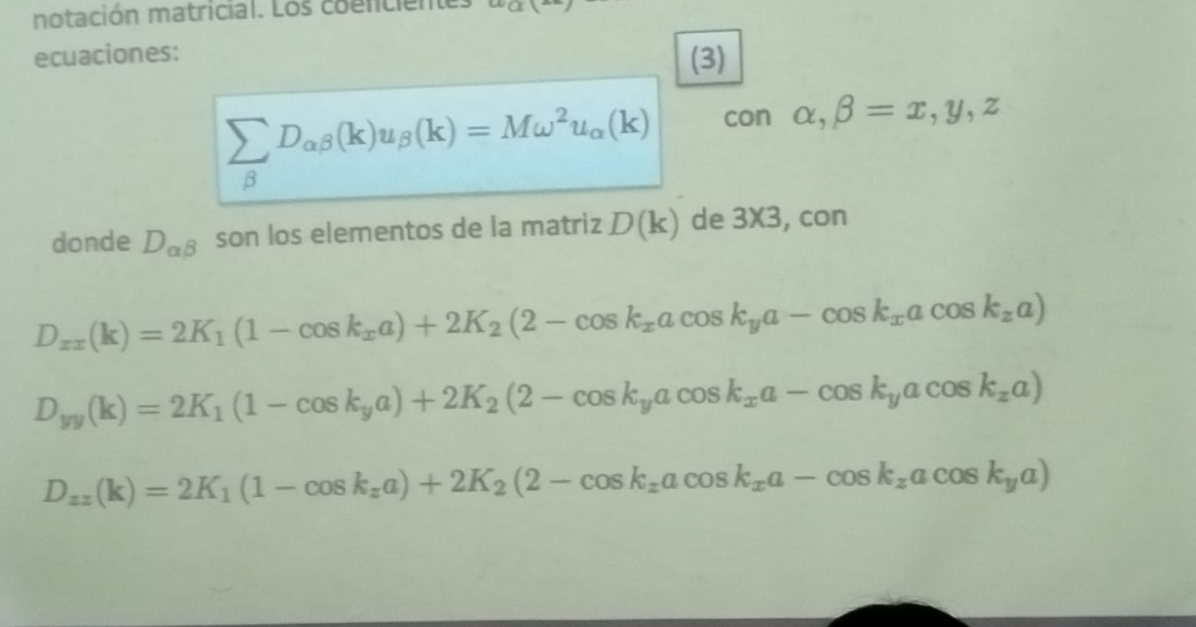
\includegraphics[width=0.7\textwidth]{12.png} % ajusta el ancho según convenga
    \caption{Descripción clara y concisa de la figura.}
    \label{fig:mi_figura} % opcional: para usar con \ref{fig:mi_figura}
\end{figure}


Si quitamos $K_{2}$ no estamos considerando segundos vecinos.

Más términos:

 \begin{figure}[H]
    \centering
    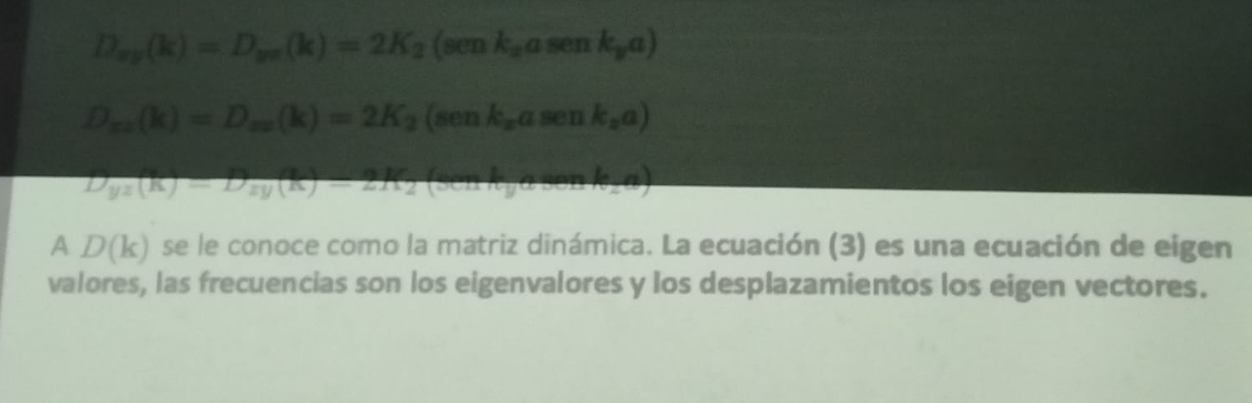
\includegraphics[width=0.7\textwidth]{13.png} % ajusta el ancho según convenga
    \caption{Descripción clara y concisa de la figura.}
    \label{fig:mi_figura} % opcional: para usar con \ref{fig:mi_figura}
\end{figure}

Análisis de las fotos anteriores.


 \begin{figure}[H]
    \centering
    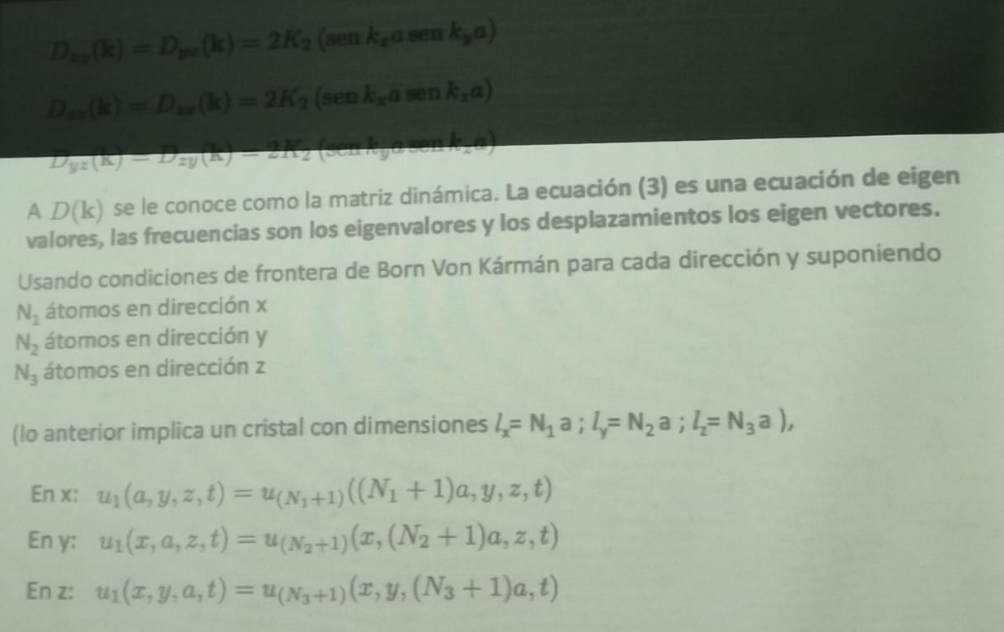
\includegraphics[width=0.7\textwidth]{14.png} % ajusta el ancho según convenga
    \caption{Descripción clara y concisa de la figura.}
    \label{fig:mi_figura} % opcional: para usar con \ref{fig:mi_figura}
\end{figure}


Valores para $k$ (dirección de propagación de la onda en ese cubo):


 \begin{figure}[H]
    \centering
	    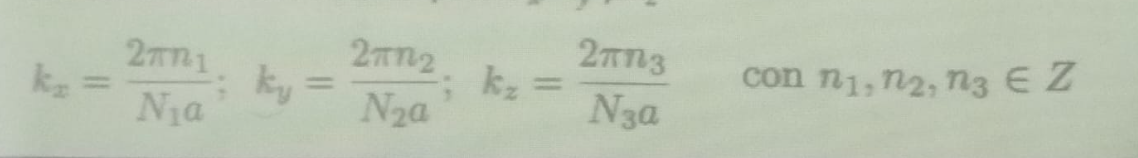
\includegraphics[width=0.7\textwidth]{15.png} % ajusta el ancho según convenga
    \caption{Descripción clara y concisa de la figura.}
    \label{fig:mi_figura} % opcional: para usar con \ref{fig:mi_figura}
\end{figure}

Es decir:

\[ \vec{k} = (k_{x},k_{y},k_{z}) \]


Tenemos considerando la 1era zona de $Brillouin$. 

\begin{figure}[H]
    \centering
	    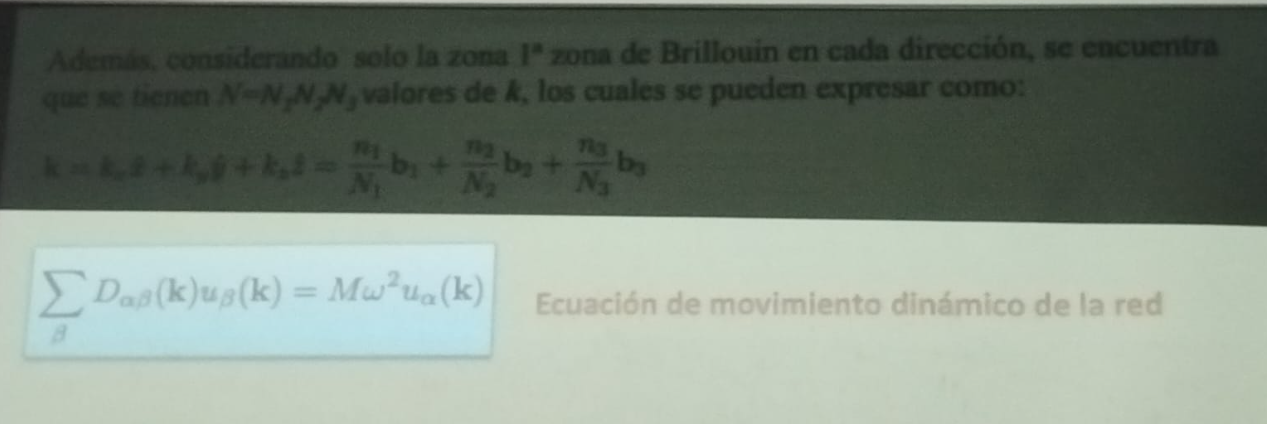
\includegraphics[width=0.7\textwidth]{16.png} % ajusta el ancho según convenga
    \caption{Descripción clara y concisa de la figura.}
    \label{fig:mi_figura} % opcional: para usar con \ref{fig:mi_figura}
\end{figure}

\textbf{Recordando problemas de \underline{eigenvalores y eigenvectores}}


\[ A\mathcal{X} = \lambda \mathcal{X}, \quad \text{con} \quad A=\text{matriz}, \mathcal{X} = \text{eigenvector}, \lambda = \text{eigenvalores} \]


Es decir, tenemos (problema general) es la ecuación \textcolor{Mahogany}{\underline{\textbf{Ecuación de movimiento dinámico de la red}}}:

\begin{figure}[H]
    \centering
	    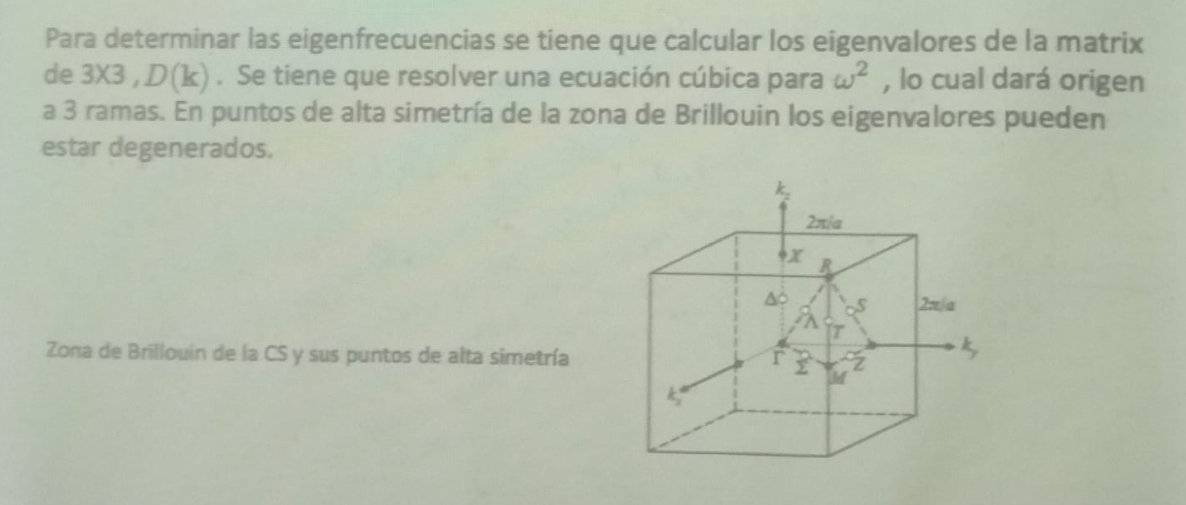
\includegraphics[width=0.7\textwidth]{17.png} % ajusta el ancho según convenga
    \caption{Descripción clara y concisa de la figura.}
    \label{fig:mi_figura} % opcional: para usar con \ref{fig:mi_figura}
\end{figure}

\begin{figure}[H]
    \centering
	    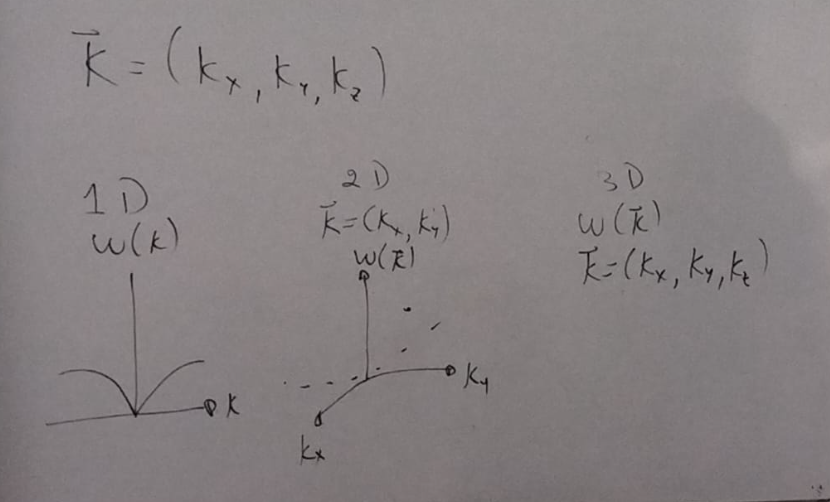
\includegraphics[width=0.7\textwidth]{18.png} % ajusta el ancho según convenga
    \caption{Descripción clara y concisa de la figura.}
    \label{fig:mi_figura} % opcional: para usar con \ref{fig:mi_figura}
\end{figure}

\begin{figure}[H]
    \centering
	    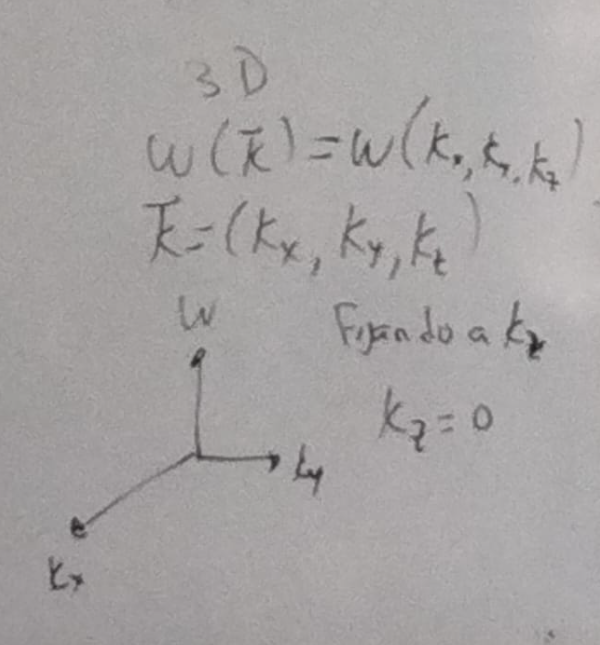
\includegraphics[width=0.7\textwidth]{19.png} % ajusta el ancho según convenga
    \caption{Descripción clara y concisa de la figura.}
    \label{fig:mi_figura} % opcional: para usar con \ref{fig:mi_figura}
\end{figure}



Recordando cómo hicimos para la cúbica (CS) construir el espacio recíproco que también es una \textbf{CS}.


Checar \textbf{notas} para ver cómo se construye la primera zona de Brillouin de la CS en el espacio recíproco. Es un cubo que tiene longitud $2\pi/a$ todo este análisis ya fue realizado en clases pasadas.

\begin{figure}[H]
    \centering
	    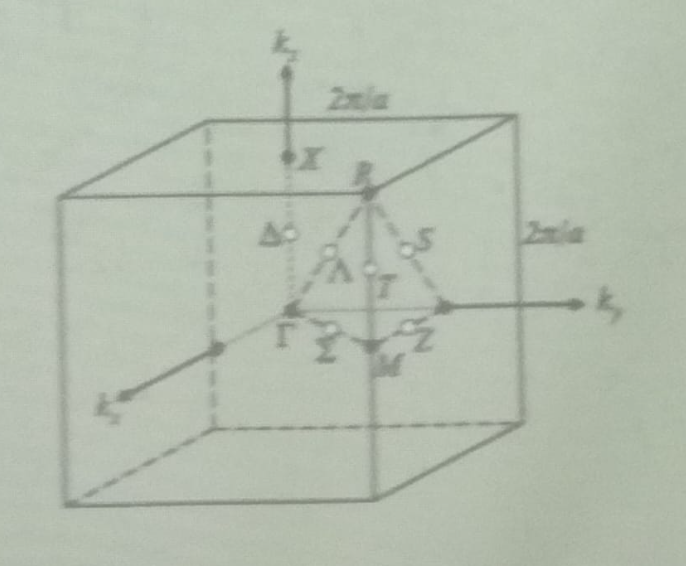
\includegraphics[width=0.7\textwidth]{20.png} % ajusta el ancho según convenga
    \caption{Descripción clara y concisa de la figura.}
    \label{fig:mi_figura} % opcional: para usar con \ref{fig:mi_figura}
\end{figure}

Tenemos buscando las coordenadas (puntos de alta simetría): 


\section*{Puntos de alta simetría en la primera zona de Brillouin}

Tenemos buscando las \textbf{coordenadas de los puntos de alta simetría} en el primer
Brillouin de una red cúbica simple (SC).  
Los vectores recíprocos están dados por:
\[
\mathbf{b}_1 = \frac{2\pi}{a}\hat{x}, \qquad 
\mathbf{b}_2 = \frac{2\pi}{a}\hat{y}, \qquad 
\mathbf{b}_3 = \frac{2\pi}{a}\hat{z}.
\]

El centro de la zona de Brillouin es el punto
\(\Gamma = (0,0,0)\), y el cubo recíproco se extiende
desde \(-\pi/a\) hasta \(+\pi/a\) en cada eje.

\subsection*{Coordenadas de los puntos principales}

En \textbf{unidades absolutas} (\(1/\text{longitud}\)):

\[
\begin{aligned}
\Gamma &= (0,\,0,\,0),\\[4pt]
X &= \left(\frac{\pi}{a},\,0,\,0\right),\\[4pt]
M &= \left(\frac{\pi}{a},\,\frac{\pi}{a},\,0\right),\\[4pt]
R &= \left(\frac{\pi}{a},\,\frac{\pi}{a},\,\frac{\pi}{a}\right).
\end{aligned}
\]

\noindent
En \textbf{coordenadas reducidas} (fracciones de \(2\pi/a\)):

\[
\begin{aligned}
\Gamma &= (0,\,0,\,0),\\[4pt]
X &= \left(\tfrac{1}{2},\,0,\,0\right),\\[4pt]
M &= \left(\tfrac{1}{2},\,\tfrac{1}{2},\,0\right),\\[4pt]
R &= \left(\tfrac{1}{2},\,\tfrac{1}{2},\,\tfrac{1}{2}\right).
\end{aligned}
\]



Cada segmento representa una dirección de alta simetría:

\[
\begin{aligned}
\Delta &: \Gamma \rightarrow X \quad [001],\\[4pt]
\Sigma &: \Gamma \rightarrow M \quad [110],\\[4pt]
\Lambda &: \Gamma \rightarrow R \quad [111].
\end{aligned}
\]

Índices de $Miller$: $[h,k,l]$

Para una red cualquiera, las coordenadas de estos puntos se pueden
obtener a partir de los vectores recíprocos mediante:
\[
\mathbf{k} = u\,\mathbf{b}_1 + v\,\mathbf{b}_2 + w\,\mathbf{b}_3,
\]
donde \(u,v,w\) toman valores fraccionarios que dependen del tipo de
red (en la cúbica simple suelen ser \(0\) o \(1/2\)).

Nos estamos moviendo en trayectorias del espacio $k$. 

Cuando tenemos rectas o curvas en el espacio \textbf{parametrizamos}. La ventaja de la parametrización es que para describir dos variables solo ocupamos un parámetros. Reducimos en número de variables en el espacio recíproco y así podamos identificar las ramas acústica y fononicas.


\begin{figure}[H]
    \centering
	    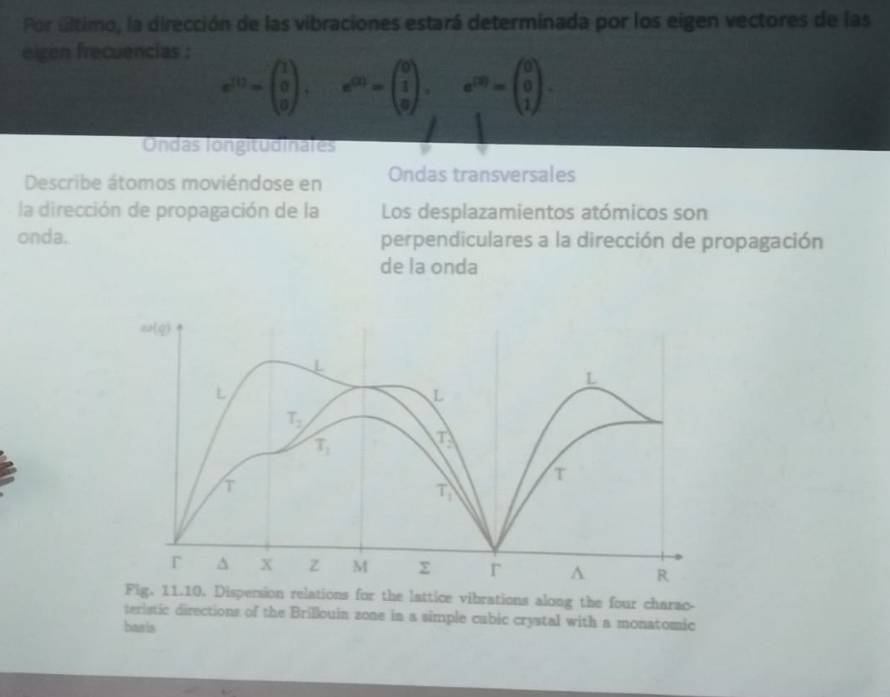
\includegraphics[width=0.7\textwidth]{21.png} % ajusta el ancho según convenga
    \caption{Descripción clara y concisa de la figura.}
    \label{fig:mi_figura} % opcional: para usar con \ref{fig:mi_figura}
\end{figure}

Alrededor del punto $\Gamma$ tiene un comportamiento muy similar a la monoatómica.


\subsection{Ejemplo} 

\emph{Veamos como ejemplo las vibraciones que se propagan en la dirección $[1,0,0]$, y que están caracterizados por el vector de onda $\Delta = (k,0,0)$.}

\begin{figure}[H]
    \centering
	    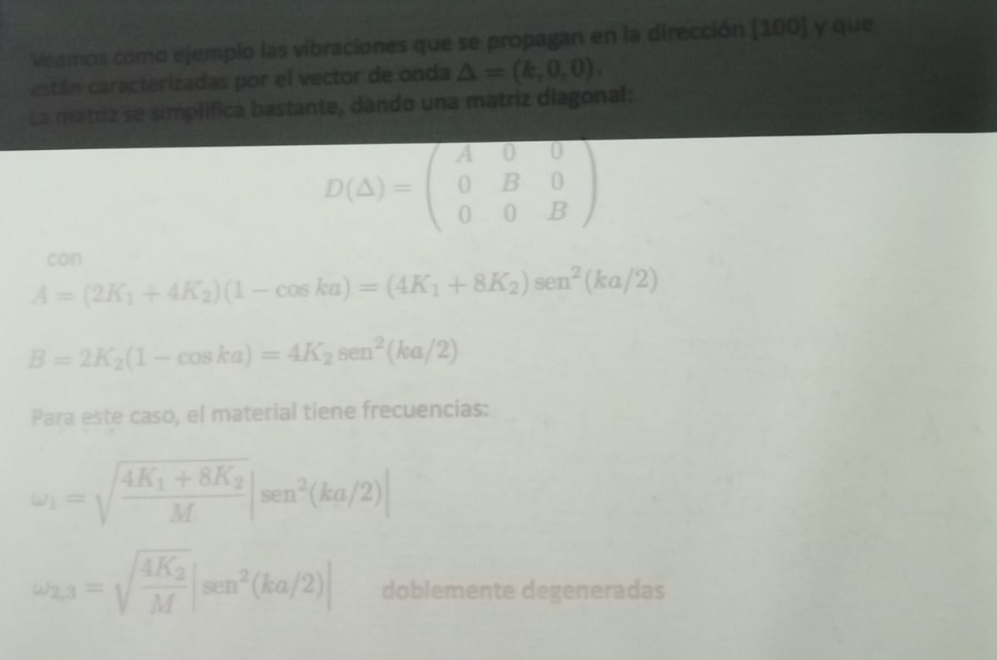
\includegraphics[width=0.7\textwidth]{22.png} % ajusta el ancho según convenga
    \caption{Descripción clara y concisa de la figura.}
    \label{fig:mi_figura} % opcional: para usar con \ref{fig:mi_figura}
\end{figure}

\textbf{OBS.} Checar las unidades para $\sen{ka/2}$ va al cuadrado o no? xd :v

\begin{figure}[H]
    \centering
	    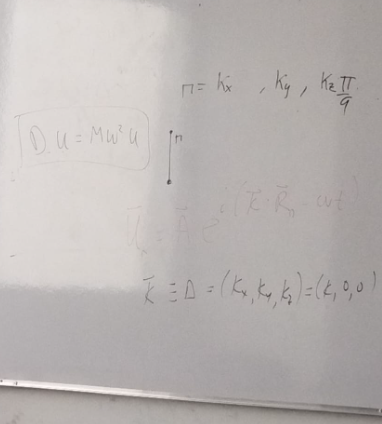
\includegraphics[width=0.7\textwidth]{23.png} % ajusta el ancho según convenga
    \caption{Descripción clara y concisa de la figura.}
    \label{fig:mi_figura} % opcional: para usar con \ref{fig:mi_figura}
\end{figure}

¿Quién define el tipo de modo normal de oscilación?

\begin{itemize}
\item[$\bullet$] Longitudinal - Los modos que tienen desplazamientos en la misma dirección de propagación
\item[$\bullet$] Transversal - Los modos que tienen desplazamientos en dirección transversal de propagación
\end{itemize}


\begin{figure}[H]
    \centering
	    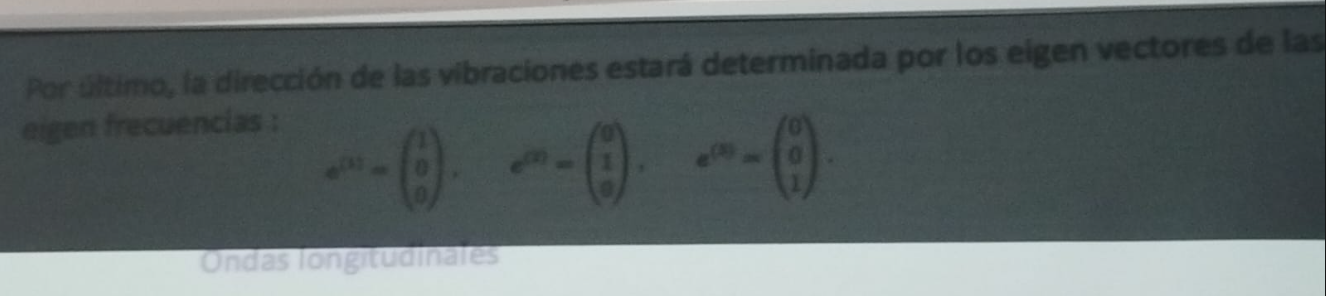
\includegraphics[width=0.7\textwidth]{24.png} % ajusta el ancho según convenga
    \caption{Descripción clara y concisa de la figura.}
    \label{fig:mi_figura} % opcional: para usar con \ref{fig:mi_figura}
\end{figure}


Si tenemos la simetría en vez de $[1,0,0] \to [0,0,1]$ tendríamos los mismos eigenvectores?

R= Sí, es alta simetría, corresponde a simetría \textbf{CS}. Está rotado.

\textbf{Tarea (teams)}:

\begin{figure}[H]
    \centering
	    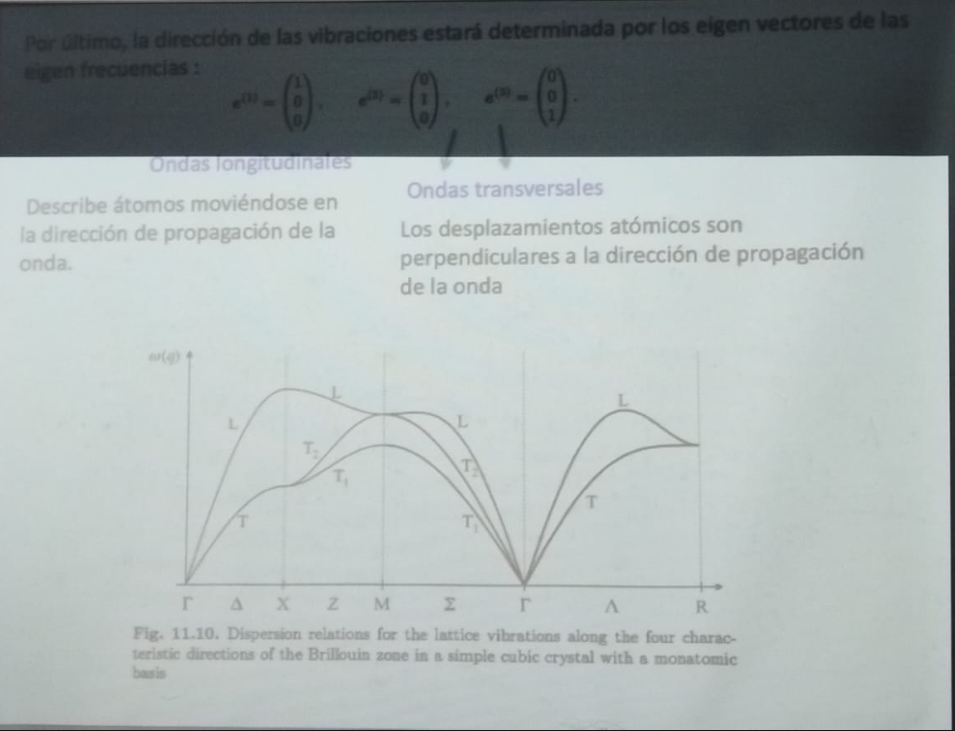
\includegraphics[width=0.7\textwidth]{25.png} % ajusta el ancho según convenga
    \caption{Descripción clara y concisa de la figura.}
    \label{fig:mi_figura} % opcional: para usar con \ref{fig:mi_figura}
\end{figure}


 






 

\end{document}